\autsection{Reaction Control System}{Søren Jeppesen}\label{chap:RCS}

The reaction control system (RCS) of the lander is the system of thrusters that control the attitude and provide minor translation control. The system uses a series of small engines to provide three-axis control of the lander to correct minor position and velocity errors, divergence from the optimal descent profile, and to to ensure that the rotational properties of the lander are ideal. The RCS is additionally to provide precise maneuvering during the landing stage to ensure safe and proper landing at the designated target.\\

This section will form an overview of the RCS envisioned for the Europa Life Finder Mission as well as some of its capabilites. A detailed schematic of the thrusters, fuel pump system, electrical power system and such will not be discussed. These design can instead be taken from already existing RCS designed for similar needs, and then modified to suit the Europa mission.

\subsection{Design}

The RCS envisioned for the Europa mission has been chosen from its similarities to lunar landing missions. As the Moons gravity is almost the same as Europas, lunar descent vehicles will serve as good inspiration for the capability needs of the RCS. Particularly, the ESA Lunar Lander and Chang'e 3 lunar descent vehicles have been used to model the RCS for the Europa mission \cite{ESA_pic} \cite{Chang_e_3}. In figure \ref{fig:landers} are seen the RCS for these missions.\\


\begin{figure}[htb]
\begin{center}
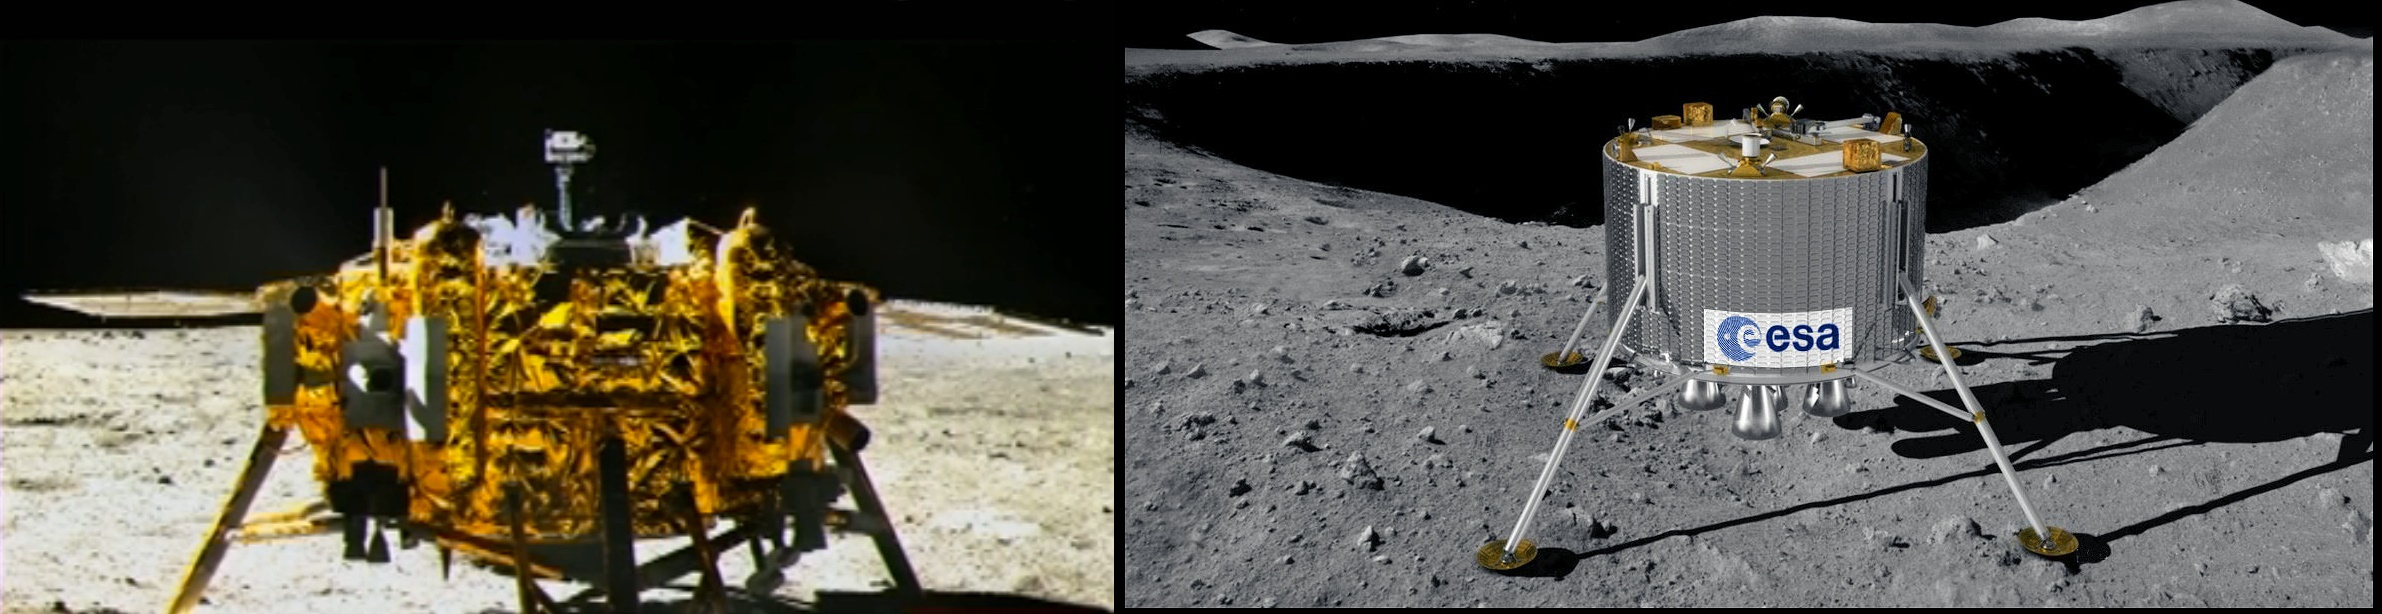
\includegraphics[scale=0.19]{figures/RCS/landers}
\caption{Image of the chinese Chang'e 3 moonlander (left). Image of the ESA Lunar Lander (right) \cite{Chang_pic} \cite{ESA_pic}}
\label{fig:landers}
\end{center}
\end{figure}


Based on these missions, the RCS for the Europa mission will consist of 16 thrusters each providing 20 N of thrust. The thrusters are positioned in four clusters of four thrusters each, positioned around the center of gravity for the lander. The total thrust output this setup can generate is larger than that of the ESA Lunar Lander, but smaller than that of Chang'e 3 \cite{ESA_pic} \cite{Chang_e_3}. This is off-set  by the differences weight. Figure \ref{fig:RCS_thruster} shows a cluster as well as a single thruster belonging to the cluster.\\

The thrusters use the green propellant as opposed to the bi-propellant used by the main engines. The properties of the propellant is outlined in the fuel section, but in short, with its high specific impulse this propellant should be well suited for the RCS without the risk of contaminating the landing site. The choice of green propellant over bi-propellant increases the difficulty of designing the RCS as most common systems use a hydrazine propellant along with an oxidizer, thus limiting the already existing schematics that can be drawn on.

\begin{figure}[htb]
\begin{center}
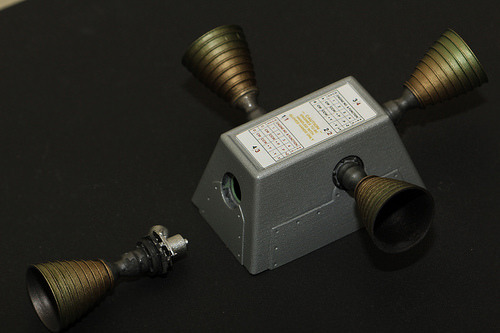
\includegraphics[scale=0.6]{figures/RCS/RCS_thruster2}
\caption{Image of an RCS thruster cluster, containing four thruster \cite{RCS_pic}}
\label{fig:RCS_thruster}
\end{center}
\end{figure}


\subsection{Rotational capabilities}

Analyzing the rotational ability of the RCS is done using a simplifed model of the lander. In this model, the moment of inertia for the lander is presented as a solid frustum cone with a solid cylinder inside. The cone represents the lander and has a uniform density throughout the volume of the cone. The cylinder inside represents the payload and has a uniform density that is different from that of the cone. Figure \ref{fig:cone} shows the model used for representing the moment of inertia.

\begin{figure}[htb]
\begin{center}
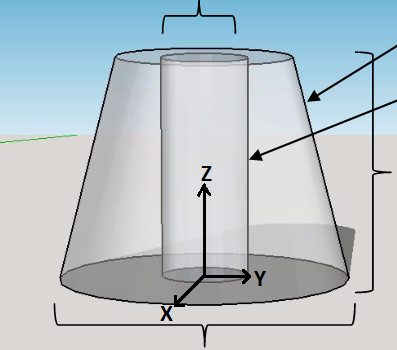
\includegraphics[scale=1]{figures/RCS/cone_payload}
\caption{3D model of the frustum cone with cylindrical payload in the middle used to describe the moment of inertia for the lander}
\label{fig:cone}
\end{center}
\end{figure}


The moment of inertia for this structure is

\begin{equation}
\begin{split}
   & I_{z} = \frac{3}{10} \cdot M_{1} \cdot R_{1}^2 - \frac{3}{10} \cdot M_{2} \cdot R_{2}^2 + \frac{1}{2} \cdot M_{diff} \cdot R_{cyl}^2\\
   & I_{y} = \frac{3}{20} \cdot M_{1} \cdot R_{1}^2 + \frac{1}{10} \cdot M_{1} \cdot h_{cone1}^2 - \frac{3}{20} \cdot M_{2} \cdot R_{2}^2\\
   &     - \frac{1}{10} \cdot M_{2} \cdot h_{cone2}^2 + \frac{1}{2} \cdot M_{diff} \cdot R_{cyl}^2
\end{split}
\end{equation}

With $I_x$ being identical to $I_y$ due to symmetry. The moment of inertia for the frustum cone is found by using the moment of inertia for a large, regular cone consisting of both the frustum cone and a smaller, regular cone. From this large, regular cone, is then subtracted the moment of inertia of the small regular cone. 

\begin{itemize}
\item $M_1$ is the mass of the large cone, which 4404.67 kg with fuel, 948.98 kg without fuel.
\item $M_2$ is the mass of the small cone, which is 1211.6 kg with fuel, 261.04 kg without fuel.
\item $R_1$ is the radius of the large cone at the bottom, which is 1 m.
\item $R_2$ is the radius of the small cone at the bottom, which is 0.6 m.
\item $h_{cone1}$ is the height of the large cone, which is 3.76 m.
\item $h_{cone2}$ is the height of the small cone, which is 2.26 m.
\item $M_{diff}$ is the difference in mass between two payload sized cylinders, where one has the density of the payload and one has the density of the rest of the lander. This value is 418.69 kg with fuel, and 51.02 kg without fuel.
\item $R_{cyl}$ is the height of the cylinder, which is 1.5 m.
\end{itemize}

The moments of inetia with fuel are then $I_{y,x}$ = 6124 $\mathrm{kg/m^2}$ and $I_{z}$ $\mathrm{kg/m^2}$ = 1188.5, and the moments of inertia without fuel are $I_{y,x}$ = 1346.3 $\mathrm{kg/m^2}$ and $I_{z}$ = 256.75. $\mathrm{kg/m^2}$ With the moment inertia, the angular acceleration of the lander can be calculated from

\begin{equation}
    I \alpha = r \times F
\end{equation}
    
here, $I$ is the moment of inertia, $\alpha$ is the angular acceleration, $R$ is the position vector of the point where the force is applied, and $F$ is the force vector. In the $x$ and $y$ directions, the RCS is capable of providing 40 N of thrust, and in the $z$ direction the RCS can proviode 80 N of thrust. The angular acceleration that the RCS can deliver is then 0.0065 $\mathrm{rad/s^2}$ in the $x$ and $y$ directions, and 0.067 $\mathrm{rad/s^2}$ in the z direction at the lower edge of the lander. This in turn makes the rotation period of the lander 43.8 s in $x$ and $y$ directions, and 13.6 s in the $z$ direction.\\

To decrease the rotation period of the lander, the thrusters can instead be placed on beams stretching out from the lander a seen on figure \ref{fig:arms}. Given 1 m long beams, the rotation period instead becomes 31.01 s in the $x$ and $y$ directions, and 9.66 in the $z$ direction.

\begin{figure}[htb]
\begin{center}
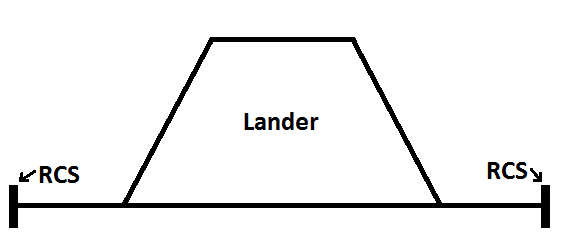
\includegraphics[scale=0.8]{figures/RCS/Lunar_arms}
\caption{Simple sketch showing the extended arms on which the RCS thrusters can be placed.}
\label{fig:arms}
\end{center}
\end{figure}

Figure \ref{fig:arms_graph} shows how the rotational acceleration of the lander increases with arm length. Using arm extensions adds additional weight to the lander. Longer arms must also  be thicker to be able to support the lander when the RCS is used.

\begin{figure}[htb]
\begin{center}
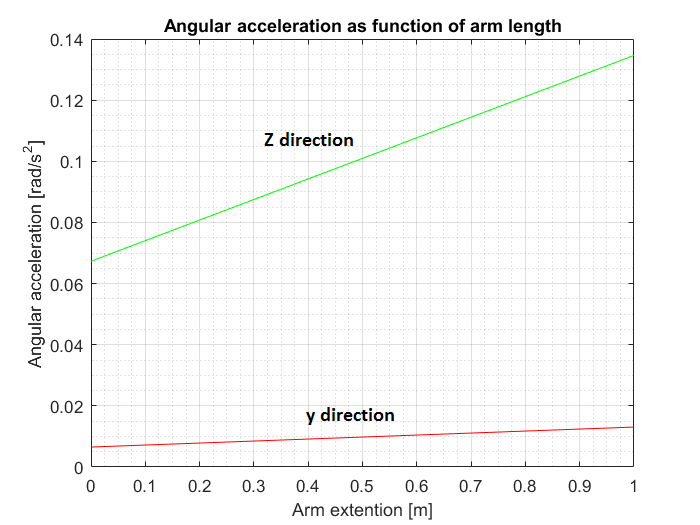
\includegraphics[scale=0.8]{figures/RCS/arm_graph}
\caption{Graph of the increase in angular acceleration of the lander due to increase in arm length.}
\label{fig:arms_graph}
\end{center}
\end{figure}

\subsection{Velocity correction}

During the descent, the lander will likely be required to make small corrections to the velocity in order to maintain optimal descent profile. With the suggested RCS, the lander will have two thrusters available for horizontal corrections (horizontal with respect to the lander), and four thrusters available for vertical corrections (with respect to the lander). With the lander sitting at 3986 kg of mass with a full fuel tank and each thruster providing 20 N of thrust, from Newton's second law of motion, the acceleration the RCS can provide horizontally is 0.01 $\mathrm{m/s^2}$, and the acceleration vertically is 0.02 $\mathrm{m/s^2}$. 

\subsection{Slide prevention}

In the final stage of the descent, the RCS can be used to prevent horizontal sliding (see figure \ref{fig:lunar_slide}) from the lander. In the case where the lander maintains upright position, the RCS provides 40 N of thrust and assuming an almost empty fuel tank, weights around 1000 kg. The RCS is then able to provide 0.04 $\mathrm{m/s^2}$ of horizontal acceleration.\\

\begin{figure}[htb]
\begin{center}
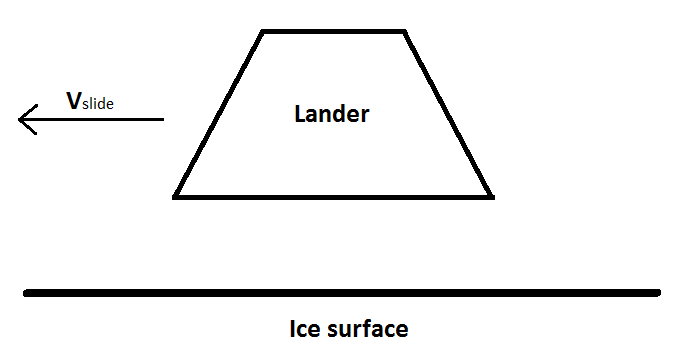
\includegraphics[scale=0.8]{figures/RCS/Lunar_slide}
\caption{Simple sketch showing the lander sliding above the ice surface with a velocity $V_{slide}$ parallel to the surface plane.}
\label{fig:lunar_slide}
\end{center}
\end{figure}

Alternatively, the lander can turn 45 degrees and activate another two thrusters to counter sliding. At this angle, each of the four sliders will provide 14.14 N of thrust in the direction opposite the sliding, for a total of 56.56 N. The horizontal acceleration is then 0.06 $\mathrm{m/s^2}$. With 10.28 seconds required to turn this angle, using this method will be more effective if the lander has a velocity parallel to the surface of 1.44 $\mathrm{m/s}$. This maneuver comes at the cost of increased fuel usage as additional thrusters must be utilized.

\begin{figure}[htb]
\begin{center}
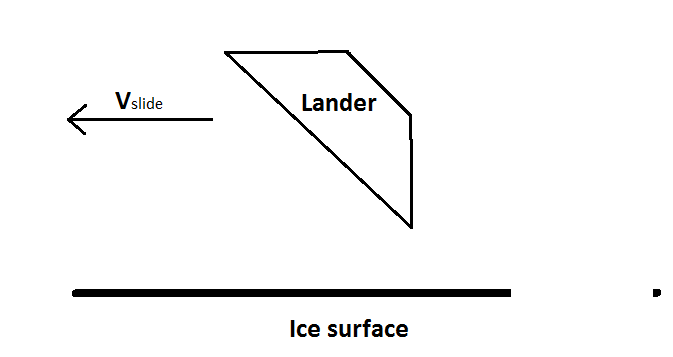
\includegraphics[scale=0.8]{figures/RCS/Lunar_slide_angle}
\caption{Simple sketch showing the extended arms on which the RCS thrusters can be placed.}
\label{fig:lunar_slide_angle}
\end{center}
\end{figure}


\subsection{Soft landing capabilities}

During the landing, the RCS must be able to maneuver the lander with high precision. To this end, the lander has eight 20 N thrusters for altitude control, providing 80 N of thrust in either upwards or downwards direction, and eight thrusters for horizontal control providing 40 N of thrust in either of the four horizontal directions. The horizontal acceleration provided by the RCS is mentioned in the previous section to be 0.04 $\mathrm{m/s^2}$, and the vertical acceleration is 0.08 $\mathrm{m/s^2}$.

\subsection{Conclusion}

An RCS for the Europa lander has been outlined in this section. The system is based on RCS from lunar landing missions such as the Chang'e 3 and ESA Lunar Lander, which have requirements similar to that of the Europa lander. Based on these similarities as well as the positional and rotational accelerations calculated, the RCS for Europa lander is thought to provide sufficient position and rotation correct, as well as soft landing. 

\subsection{Further work}

Several relevant topics on the RCS still needs to be discussed. As this section only briefly introduces the RCS, the technical details such the power system, fuel pump system, and thruster design has been left out of this. The rotational capabilities of the system has been calculated from a very simplified model of the lander. In truth, the lander is much more complex in shape and weight distribution than the model implies, and it would be relevant to investigate how a more correct model would fare, and how the thrusters should be positioned for optimal use.
